% Appendix A

\chapter{Feedforward Neural Networks} % Main appendix title

\label{AppendixA} % For referencing this appendix elsewhere, use \ref{AppendixA}

\textcolor{red} {[TODO: Introduce FFNs] }

\section{Terminology}

Figure~\ref{fig:Terminology} presents the terminology in a FNN with three input signals, a hidden layer with two neurons, and one output signal.

\begin{figure}[h]
	\centering
	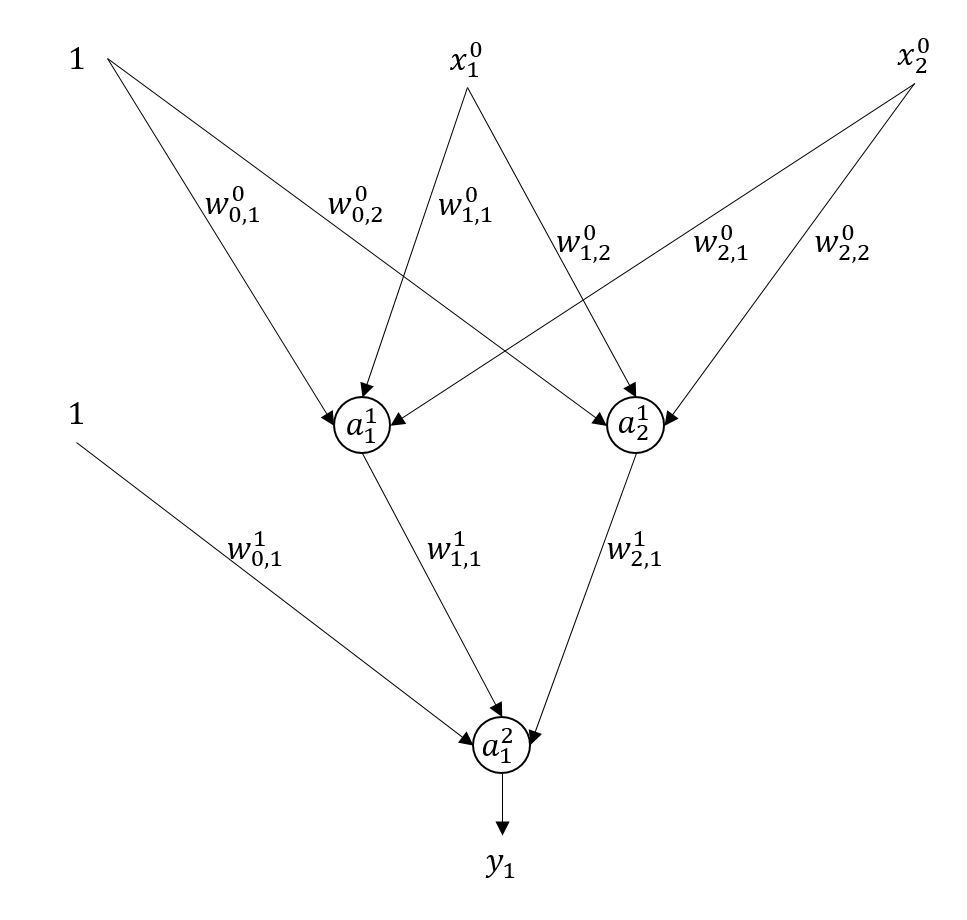
\includegraphics{Figures/ffn_v1.PNG}
	\decoRule
	\caption[Neural Networks Terminology]{Neural Networks Terminology}
	\label{fig:Terminology}
\end{figure} 


In this terminology figure $w^{m}_{ij}$ represents the weight in the synaptic link that joins neuron $a^{m}_{i}$ with neuron $a^{m+1}_{j}$. Also $m$ indicates the layer in the neural network, where the input layer has $m=0$, and the output layer $m=2$. The two input signals are given by $x^{0}_{1}, x^{0}_{2}$, and the output signal by $y_1$. Even though it is not shown in the figure, the output of the hidden neurons  $a^{1}_{1}$ and $a^{1}_{2}$ are $x^{1}_{1}$ and $x^{1}_{2}$ respectively.

\section{Backpropagation Training in FNNs}
Supervised training of FNNs can be done through the backpropagation method, which consists in propagating the output error with respect to the training data down all the internal layers in the network in order to adjust the weights while optimizing a model.
\\
\subsection{Mean Square Error}
The weights in a neural network are initialized to random values, and then modified through gradient descent methods to reduce a given error function between $k$ real ($y$) and predicted ($y^*$) output values. 
\\
The mean square is an example of an error function that can be used.

\begin{equation}\label{eq:3}
E= \sum_{i=1}^{k} E_i =\frac{1}{2}\sum_{i=1}^{k}(y_i^* - y_i)^2
\end{equation}
\\
The optimization of the weights in a neural network requires the calculation of the gradient of the error function with respect to each of the weights.




\textcolor{red} {[TODO: Add explanation of backpropagation training here] }